\chapter{Numerical Methodology and CFD Simulations}
\label{ch:numerics}

This chapter documents the simulations as they were run. Settings were taken from the Fluent report files that came with the results (\texttt{report.xml}) and from screenshots of the solver set-up. Where a setting is not documented, this is stated rather than assumed.

\section{Computational set-up}

\paragraph{Geometry preparation.} The planform of \cref{fig:geometry} was generated by a Python script (CadQuery) and exported as a STEP solid of height \SI{145}{\micro\metre}. The hyperbolic walls are single splines through 241 points, not polylines, which avoids the many small faces that polyline imports produce. The ports of the physical chip (3 and \SI{1.5}{mm} punched holes) were not modelled. Inflow enters through the face of the lead-in and outflow leaves through the face of the outlet duct. Named selections (\texttt{inlet}, \texttt{outlet}, walls) were defined before meshing.

\paragraph{Computational domain.} The domain is the full three-dimensional fluid volume (\SI{20.745}{\milli\metre\cubed}), without symmetry planes. The PDMS and the glass were not meshed; they enter the flow problem only as no-slip walls.

\paragraph{Mesh.} The mesh files and the mesh statistics were not included in the results we received, so the element type, the cell count and the quality metrics are not documented (\cref{app:missing}). Two properties can be inferred from the exported data:
\begin{enumerate}
\item \emph{Resolution across the gap.} In each cross-section the interior nodes carry four distinct velocity values, each appearing twice, for example 0.046, 0.091, 0.130 and \SI{0.160}{mm/s} per \ulmin\ at S1. This is the signature of eight interior node levels placed symmetrically about the mid-plane, i.e.\ about \textbf{nine cell layers across the \SI{145}{\micro\metre} gap}, slightly graded towards the walls.
\item \emph{Resolution near the side walls.} Wall nodes are \SIrange{0.08}{0.10}{mm} apart next to the side walls (\cref{tab:transverse_nodes}). This is comparable to the theoretical side-wall layer of \SI{0.129}{mm}, so the layer is only marginally resolved.
\end{enumerate}
No mesh images are available. The flow-rate cases used the same mesh: the number of nodes in every exported cross-section is identical in all three cases.

\paragraph{Mesh independence.} Only one mesh was run, so mesh independence could not be demonstrated. A study has been designed (\cref{sec:num_gci}) but not yet carried out. This is the most important open point of the validation (\cref{sec:val_offset}).

\section{Solver set-up}
\label{sec:num_solver}

\Cref{tab:solver} lists the solver settings.

\begin{table}[htbp]
\centering
\caption{ANSYS Fluent settings of the present simulations \tagC, from \texttt{report.xml} unless stated.}
\label{tab:solver}
\small
\begin{tabularx}{\linewidth}{@{}p{0.3\linewidth}X@{}}
\toprule
Setting & Value\\
\midrule
Software & ANSYS Fluent 2024 R1 (24.1.0), 3D, double precision\\
Formulation & Pressure-based, \textbf{steady}\\
Viscous model & Laminar; energy equation off (isothermal)\\
Material & Constant $\rho=\SI{981.8}{kg/m^3}$, $\mu=\SI{0.00094}{Pa.s}$ (medium at \SI{37}{\celsius} \citep{Delon2020})\\
Pressure--velocity coupling & SIMPLEC\\
Spatial discretisation & Pressure: PRESTO!; momentum: second-order upwind\\
Gradient method & Not contained in the exported report (Fluent default: least-squares cell-based)\\
Under-relaxation & Pressure 0.3, momentum 0.7\\
Gravity & Off (modified pressure, \cref{ch:governing})\\
Initialisation & Not documented\\
Convergence control & See \cref{sec:num_convergence}\\
\bottomrule
\end{tabularx}
\end{table}

Two choices differ from the reference paper. First, the paper ran a transient simulation with a time step of \SI{e-7}{s} to observe how the flow develops. Here a steady formulation was used, because the boundary conditions are constant, the viscous adjustment time is \SI{0.022}{s}, and only the steady state is analysed in both studies. Second, SIMPLEC replaces SIMPLE; both converge to the same steady solution, SIMPLEC usually in fewer iterations \citep{Patankar1980,Fluent2024}. PRESTO! interpolates pressure at the faces using a staggered-type stencil, which suits the strong pressure gradients normal to thin layers. Second-order upwind reduces numerical diffusion. At these Reynolds numbers convection is negligible in any case, so the choice of convection scheme has almost no effect on the flow.

\section{Convergence monitoring}
\label{sec:num_convergence}

The first runs used Fluent's \emph{absolute} residual criteria of $10^{-6}$ for continuity and the three momentum equations (\cref{fig:residuals}a), and the solver reported convergence after three iterations, with residuals printed as zero (\cref{fig:residuals}c; that console run also had the energy equation listed, so it predates the final set-up). This is not a meaningful convergence. At a mass flow of \SI{3.6e-9}{kg/s}, all fluxes in the domain are tiny, so the residuals start below an absolute threshold that was designed for flows of order \si{kg/s}. The settings were then changed (\cref{fig:residuals}b): the convergence criterion was set to \emph{none}, normalised and scaled residuals were plotted, and the solution was iterated until monitored physical quantities stopped changing.

\begin{figure}[htbp]
\centering
\begin{subfigure}[t]{0.47\linewidth}\centering
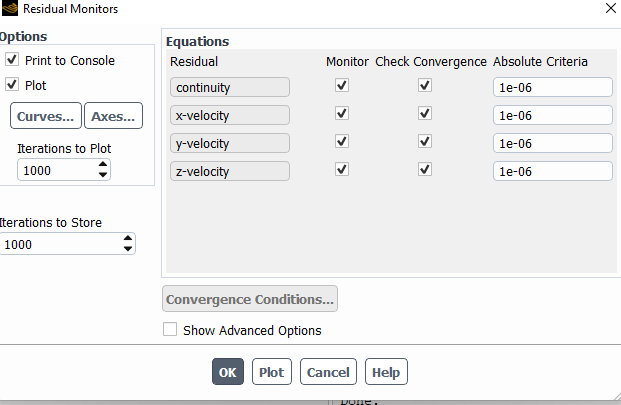
\includegraphics[width=\linewidth]{fluent_residuals_absolute.png}
\caption{Initial: absolute criteria $10^{-6}$.}
\end{subfigure}\hfill
\begin{subfigure}[t]{0.5\linewidth}\centering
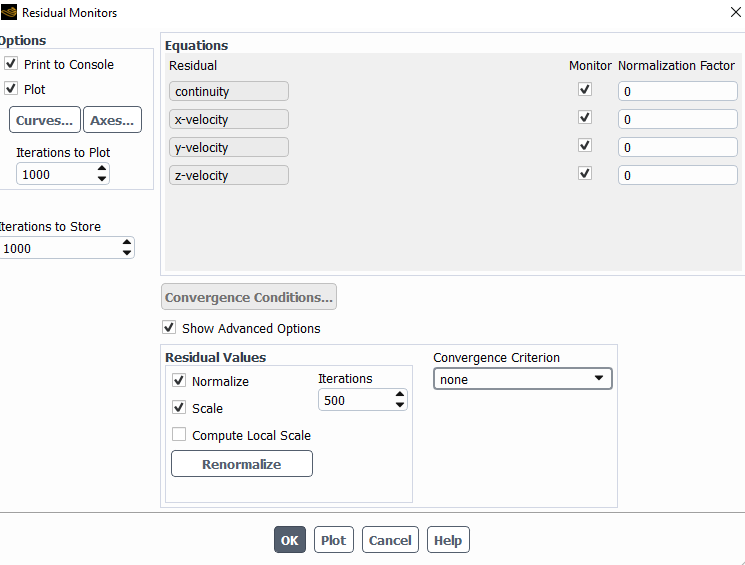
\includegraphics[width=\linewidth]{fluent_residuals_none.png}
\caption{Revised: criterion ``none'', normalised and scaled.}
\end{subfigure}

\vspace{2mm}
\begin{subfigure}[t]{0.75\linewidth}\centering
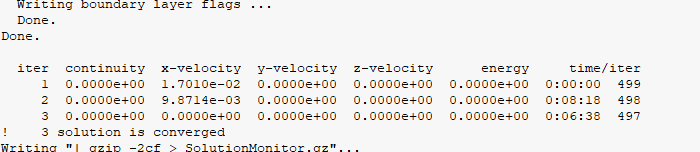
\includegraphics[width=\linewidth]{fluent_console_3iter.png}
\caption{Console message obtained with the initial settings.}
\end{subfigure}
\caption{Residual-monitor settings used during the project (screenshots from Fluent). With absolute criteria the very small fluxes of a \si{\micro\litre\per\minute} flow satisfied the criterion after three iterations. The revised settings rely on monitored quantities instead.}
\label{fig:residuals}
\end{figure}

The documents we received do not show which of the two settings produced the exported results, and they contain no residual history and no mass-flux report. Convergence therefore has to be judged from the results themselves. Four observations indicate a converged solution:
\begin{enumerate}
\item the pressure decreases monotonically at all 730 axial positions, in all three cases;
\item the wall shear and the pressure gradient obey the momentum balance $\taw=(h/2)|\dd p/\dd x|$ to within \SI{0.8}{\percent} (\cref{tab:momentum});
\item the three flow rates, which span a factor of 545, give results proportional to $Q$ to within \SI{0.08}{\percent} (\cref{sec:val_scaling}); solutions stopped at different stages of convergence would be unlikely to agree this closely;
\item the floor and lid shear agree to \SIrange{0.1}{0.8}{\percent}, as the mid-plane symmetry requires.
\end{enumerate}
The inlet/outlet mass balance (\emph{Reports $\to$ Fluxes}) should still be reported, because it is the only direct test of mass conservation.

\section{Boundary conditions}

\begin{table}[htbp]
\centering
\caption{Boundary conditions of the flow simulations \tagC.}
\label{tab:bc}
\small
\begin{tabularx}{\linewidth}{@{}p{0.1\linewidth}p{0.14\linewidth}p{0.26\linewidth}X@{}}
\toprule
Boundary & Fluent type & Value & Physical reasoning\\
\midrule
\texttt{inlet} & mass-flow inlet & $\dot m=\num{3.6e-9}$, \num{1.636e-8}, \SI{1.964e-6}{kg/s} (normal to face) & A syringe pump imposes the flow rate; $Q=\dot m/\rho=0.2200$, 0.9998, \SI{120.02}{\uLmin}. The face receives a uniform velocity, which develops into the duct profile within \SI{0.09}{mm}, far upstream of $x=0$.\\
\texttt{outlet} & pressure outlet & \SI{0}{Pa} gauge & Outlet port open to the reservoir at atmospheric pressure; only pressure differences matter in incompressible flow.\\
all walls & stationary wall & no slip, $\vect u=\vect 0$ & Continuum liquid on solid walls ($Kn\sim10^{-6}$).\\
\bottomrule
\end{tabularx}
\end{table}

The turbulence intensity and hydraulic diameter that Fluent requests at inlets and outlets are irrelevant for a laminar model and were left at their defaults. The uniform inlet velocity creates a local shear peak at the inlet face of the lead-in, which dominates the colour scale of the wall-shear contours (\cref{fig:contours}). Because the lead-in is \SI{2}{mm} long, more than 20 development lengths, this peak does not affect the hyperbolic section.

\section{Exported data}
\label{sec:num_exports}

For each flow rate, twelve Fluent XY exports were analysed:
\begin{itemize}
\item static pressure and wall shear stress along the axis ($0\le x\le\SI{50.25}{mm}$, 740 points on a wall at $y=0$);
\item wall shear stress at the five stations, on the plane $x=$ const, against $y$;
\item velocity magnitude at the five stations, on the plane $x=$ const, against $y$.
\end{itemize}
Two features of these exports constrain the analysis:
\begin{enumerate}
\item The cross-section exports contain the nodes of a whole plane plotted against $y$, at all heights, without the $z$ coordinate. Wall shear is non-zero only at the wall nodes, and these come in near-coincident floor/lid pairs. The velocity is the magnitude $|\vect u|$, not $u_x$. The parabolic profile $u_x(z)$ therefore cannot be reconstructed.
\item The axial line lies on a wall at $y=0$. Whether it is the floor or the lid cannot be told from the data, but by symmetry the two agree to within \SI{0.8}{\percent}.
\end{enumerate}
The raw files were parsed from their headers and kept unchanged. Duplicated positions were averaged only for interpolation and differentiation. Local pressure gradients were obtained by least-squares regression over a $\pm\SI{0.4}{mm}$ window, and station values by linear interpolation. The post-processing scripts are listed in \cref{app:repro}.

\section{Numerical reliability}

\paragraph{What has been established.} Iterative convergence is supported by the internal consistency checks listed above. Mass conservation in the integral sense is supported by the exact scaling with $Q$, but it has not been checked directly. The simulations are numerically stable: they show no oscillation, no backflow and no non-monotonic pressure.

\paragraph{What has not been established.} The magnitude of the discretisation error is unknown. \Cref{ch:validation} will show a uniform \SI{-5}{\percent} offset of shear and pressure gradient relative to the side-wall-corrected theory. Its most probable cause is the limited number of cells across the gap. With nine layers, a one-dimensional finite-volume estimate already under-predicts the wall gradient by \SI{2.4}{\percent}, and graded, unstructured three-dimensional cells with node-value interpolation can plausibly double this. Other error sources are:
\begin{itemize}
\item node-to-node fluctuations of about $\pm\SI{1}{\percent}$ in exported wall values on an unstructured surface mesh;
\item corner nodes that average adjacent wall faces;
\item the marginal resolution of the side-wall layer;
\item the inferred, rather than documented, channel height and lead-in.
\end{itemize}

\subsection{Planned mesh-independence study}
\label{sec:num_gci}

A two-factor study at \SI{1}{\uLmin} has been prepared on swept hexahedral meshes (an all-quad face mesh on the floor swept across the gap):
\begin{itemize}
\item \emph{Study A} varies the number of layers across the gap, $N_z=9$, 18 and 36, at an in-plane size of \SI{50}{\micro\metre};
\item \emph{Study B} varies the in-plane size, $\Delta s=100$, 50 and \SI{25}{\micro\metre}, at $N_z=18$.
\end{itemize}
Both use a refinement ratio $r=2$. For a quantity $\phi$ on fine, medium and coarse meshes ($\phi_1,\phi_2,\phi_3$), the grid convergence index \citep{Roache1994,Celik2008} is computed from
\begin{equation}
p=\frac{\ln|(\phi_3-\phi_2)/(\phi_2-\phi_1)|}{\ln r},\qquad
\phi_{\mathrm{ext}}=\frac{r^p\phi_1-\phi_2}{r^p-1},\qquad
\mathrm{GCI}_{\mathrm{fine}}=\frac{F_s\,|(\phi_2-\phi_1)/\phi_1|}{r^p-1},
\label{eq:num_gci}
\end{equation}
with $F_s=1.25$. A quantity is accepted only if the following hold:
\begin{itemize}
\item the convergence is monotonic;
\item the observed order $p$ is between 1 and 3;
\item the asymptotic ratio is close to 1;
\item $\mathrm{GCI}_{\mathrm{fine}}$ is below \SI{1}{\percent}.
\end{itemize}
The quantities tracked are $\taw$ at S1--S5, $\Delta p$ and the peak velocity at S3. If $\taw$ rises towards T2 as $N_z$ increases, the \SI{-5}{\percent} offset is discretisation error. If it does not, the offset has another cause.
